\documentclass[conference]{IEEEtran}

% The preceding line is only needed to identify funding in the first footnote. If that is unneeded, please comment it out.
\usepackage{cite}
\usepackage{changepage}
\usepackage[T1]{fontenc}
\usepackage{amsmath,amssymb,amsfonts}
%\usepackage{bbold}
\usepackage[export]{adjustbox}
\usepackage{algorithmic}
\usepackage{graphicx}
\usepackage{float}
\usepackage{graphbox}
\usepackage{textcomp}
\PassOptionsToPackage{hyphens}{url}\usepackage{hyperref}
\usepackage{xcolor,colortbl}
\usepackage{dblfloatfix}
\newcommand{\cbox}[1]{\raisebox{\depth}{\fcolorbox{black}{#1}{\null}}}
\newcommand{\n}{\hfill\break}
%\usepackage{svg}

\usepackage{eso-pic}
\usepackage{pict2e}
\hypersetup{
	colorlinks,
	linkcolor={red!50!black},
	citecolor={green!75!black},
	urlcolor={blue!80!black}
}
\def\BibTeX{{\rm B\kern-.05em{\sc i\kern-.025em b}\kern-.08em
    T\kern-.1667em\lower.7ex\hbox{E}\kern-.125emX}}
\begin{document}
\makeatletter
\newlength{\logoheight}
\setlength{\logoheight}{50pt} % set your logo height
\author{\IEEEauthorblockN{Jesse McDonald}
	\IEEEauthorblockA{
		745 Paani Street,
		Unit A,
		Honolulu, HI $\cdot$ (208)553-4263 $\cdot$
		jamcdonald120@gmail.com
	}
}

\title{\parbox[c]{.75\linewidth}{{\fontfamily{bch}\selectfont\Huge{\textbf{Journal of Cosmere Science}}\\\huge{Volume 1}}}% used parbox to have multiple lines available
    \hfill% to put the logo on the right
    \raisebox{\dimexpr-.5\logoheight+.5ex\relax}% This aligns the logo vertically 
    {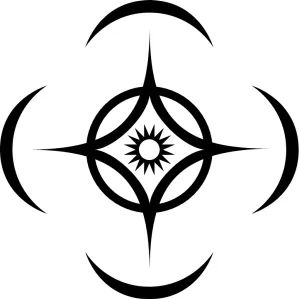
\includegraphics[height=\logoheight]{images/cosmere_symbol.png}}\par% your logo
    \vspace{15pt}% Space between logo and Title
    
    \hrule
}

\onecolumn
\maketitle{}

\begin{adjustwidth}{40pt}{80pt}
\noindent{}February 7, 2023\\

\noindent{}Brandon Sanderson\\
Prime Researcher\\
Dragonsteel Entertainment\\
Pleasant Grove, UT 84062\\

\noindent{}Dear Dr. Sanderson,\\

Over the past 8 months I have been working on an academic paper summarizing everything known about the 3 metallic arts in the Cosmere.  This paper is written as though the Cosmere is a real place that you have visited, and your books are merely recountings of the things you have seen.  At its inception, I had intended to also create an online ``Academic'' Journal for other people too also submit papers to for peer review and publication.  Regrettably such a platform is currently out of my resource set, but I have not given up hope for it, and still intend to get it up and running one day (possibly a good project for Ben).\\

In any case I wrote this paper in anticipation of The Lost Metal as a refresher.  I nearly finished it in time too, and I published an early copy on Reddit.  But then TLM happened, and we all know some revisions had to happen now don't we.  I have spent the time since then finishing up the Citations, and polishing the format, oh and adding details from Tress.  I think it is finally finished.\\

Unfortunately I have not been able to get anyone ot Peer edit it, but I believe all of my facts are cited, and my speculations reasonable.  However, there may be some incorrect assumptions I am making.\\

I do hope you and your team enjoy this work, and would greatly appreciate (but do not expect) you to review it for accuracy.  Use it however you wish.\\

Say hi to Hoid and Kriss for me next time you see them.\\


\end{adjustwidth}
\vspace{\fill}
\begin{adjustwidth}{100pt}{00pt}
	\noindent{}Best Wishes,\\\\\\\\
	
	
	
	\noindent{}Jesse McDonald\\ Copperkeep
\end{adjustwidth}
\clearpage
\begin{figure}
\begin{center}
	\vspace*{15pt}
\fontfamily{bch}\fontsize{40}{50}\selectfont{\textbf{Journal of Cosmere Science\\}}\vspace{30pt}

\includegraphics[width=\textwidth,align=c]{images/cosmere_symbol_max.png}\\\vspace{30pt}
\fontfamily{bch}\fontsize{20}{30}\selectfont{Volume 1\\}

\includegraphics[width=70pt,right]{images/digital_version.png}
\small{}Digital version available at https://github.com/Jamcdonald120/Cosmere-Peer-Edited-Journal/releases/tag/Volume-1

\end{center}
\end{figure}
%\AddToShipoutPictureFG{%
%	\AtPageLowerLeft{%
%		\Line(\LenToUnit{\paperwidth},0)(0,\LenToUnit{\paperheight})%
%		\Line(\LenToUnit{\paperwidth},\LenToUnit{\paperheight})(0,0)%
%	}%
%}
\end{document}

